\documentclass[12pt,oneside]{book}
\usepackage[utf8]{inputenc}
\usepackage[T1]{fontenc}
\usepackage{lmodern}
\usepackage{amsmath,amssymb}
\usepackage{graphicx}
\usepackage{hyperref}
\usepackage{geometry}
\usepackage{setspace}
\usepackage{tocbibind}
\usepackage{physics}
\usepackage{csquotes}
\usepackage{siunitx}
\usepackage{booktabs}
\geometry{letterpaper,margin=1in}
\onehalfspacing
\usepackage{tikz}
\usepackage{pgfplots}
\pgfplotsset{compat=newest} 
\usetikzlibrary{calc}
\usetikzlibrary{pgfplots.fillbetween}
\usepackage{tabularx}
\usepackage[backend=biber,style=numeric]{biblatex}
\addbibresource{references.bib}
\usepackage{listings}
\usepackage{xcolor}
\usepackage{physics}


\title{Gravity as Time: \\
{A Scalar-Field Framework for Gravitation and Quantum Evolution}}
\author{E.F.G. Herrera}
\date{May 2025}

\newenvironment{dedication}{\clearpage\thispagestyle{empty}\vspace*{4cm}\begin{flushright}\itshape}{\end{flushright}\vfill\clearpage}


\begin{document}
\frontmatter

\begin{titlepage}
  \centering
  {\LARGE Gravity as Time\\[0.5em] \Large A Scalar‑Field Framework for Gravitation and Quantum Evolution\par}
  \vspace{3cm}
  {\large © 2025 E. F. G. Herrera\\Valenzuela, Philippines\\\texttt{codeherrera333@gmail.com}\par}
  \vfill
  First edition, May 2025
\end{titlepage}

\thispagestyle{empty}
\noindent
All rights reserved. No part of this publication may be reproduced, stored in a retrieval system, or transmitted in any form or by any means—electronic, mechanical, photocopying, recording, or otherwise—without the prior written permission of the author, except for brief quotations used in critical articles or reviews.
\vfill
\clearpage

\begin{dedication}
To all who find new rhythms in the ticking of the Universe.
\end{dedication}

\chapter*{Preface}
I wrote this paper out of pure curiosity. It was not for school, a job or anyone else's expectations, just a quiet pursuit of something that genuinely fascinated me. Along the way, I found myself drawing inspiration from the minds of Leonardo da Vinci, Albert Einstein, and the wisdom of Tao Te Ching. Their ways of thinking helped me unlock a creative space that felt natural, unforced, and deeply personal. \\
\\
Da Vinci, for example, didn’t rush his work. Some of his paintings remained unfinished not because of laziness, but because he refused to force creativity. Leonardo da Vinci could watch ripples in a pond for an hour and call it a good day’s work. He followed his natural curiosity instead of rigid plans, letting ideas unfold through careful observation of nature. Einstein, on the other hand, played with ideas through vivid thought experiments. He trusted his intuition deeply. One of his quotes stayed with me throughout this journey:\\

\begin{displayquote}
\itshape
"Imagination is more important than knowledge. 
For knowledge is limited to all we now know and understand,
while imagination embraces the entire world, and all there ever will be to know and understand."
\end{displayquote}

\hfill—\, Albert Einstein \\
\\
These ideas resonated with something I found in the \emph{Tao Te Ching}, especially the concept of \emph{wu wei} acting without force, flowing with the nature of things. It’s not about being idle or lazy, but about moving through life in a way that feels aligned, intuitive, and honest. That spoke to me. \\
\\
Today’s world often praises relentless productivity, linear careers, and constant “hustle.” But I don’t feel like I belong to that mold. I don’t enjoy the idea of a job just for security’s sake. In fact, I wrote this paper in secret. My parents want me to have a stable job, so I pretend to do something that sounds like work just so they won’t worry. But deep down, I crave a simpler life. One where I can be myself. One where I’m not following someone else’s path.\\
\\
This paper may not be perfect but it is a reflection of a small act of curiosity, honesty, and creative freedom.

\chapter*{Abstract}
We propose that gravity arises not from curvature of spacetime but from curvature of a scalar time field~$\tau(x)$. 
Starting with a diffeomorphism‑invariant action containing a kinetic term, a light mass $m_\tau\approx10^{-28}\,\si{eV}$, 
and a weak quartic self‑interaction~$\lambda$, variation yields the field equation
\begin{equation}
  \Box\tau=\kappa T,\qquad \kappa=\frac{8\pi G}{c^{4}}.
\end{equation}
The theory reproduces the four classical Solar‑System tests, delivers post‑Newtonian parameters 
$\gamma=\beta=1$ with vanishing preferred‑frame coefficients, and matches super‑nova distance moduli to 
\SI{0.04}{mag} without dark energy. A Yukawa‑suppressed self‑interaction lets~$\tau$ explain the Bullet‑Cluster 
mass–gas offset while remaining invisible in the Solar System. Quantum‑mechanically, replacing $t\to\tau$ predicts
 altitude‑dependent tunnelling delays at the $10^{-15}$ level. All simulation code is open source; the framework is 
 therefore falsifiable by forthcoming clock‑network, weak‑lensing, and gravitational‑wave observations.


\tableofcontents
\clearpage
\listoffigures  
\clearpage

\mainmatter

\chapter*{Introduction}
\addcontentsline{toc}{chapter}{Introduction}
\markboth{Introduction}{Introduction}

Gravity as Time re imagines gravity not as the bending of a four-dimensional fabric, but as the bending of time itself. 
Instead of thinking of space curving around planets and stars, imagine that every point in the Universe carries its own 
little clock. Where there's more mass (like near a planet or a black hole), that local clock runs more slowly; where there's
less mass, it runs faster. Objects then “fall” toward massive bodies simply because they move from 
regions of faster ticking to slower ticking much like water flowing down a pressure gradient.

This single “clock field” $\tau$ carries all of gravity's information. In everyday situations, planets 
orbiting the Sun, light bending around the Earth, radar signals taking extra time to skim past the 
Sun, these effects emerge exactly as in Einstein's theory, but without needing ten components of a curved spacetime. 
In the cosmic arena, the same slowing-time picture reproduces the observed acceleration of distant super-novae 
and galaxy surveys without calling on mysterious “dark energy.” It even forms invisible halos around colliding 
galaxy clusters that mimic the behaviour normally attributed to dark matter.

On the quantum side, replacing the universal time parameter with the local clock field $\tau$ makes new, concrete predictions. 
Tiny differences in how quickly time flows at different heights on Earth would subtly alter the rate at which quantum 
particles tunnel through barriers, a shift so small (parts in $10^{15}$) that it's just within reach of today's most precise 
atomic clocks and SQUID detectors. Likewise, this framework predicts a single “breathing” mode of gravitational 
waves, distinct from the two tensor modes LIGO already sees and upcoming observing runs could confirm or rule it out.
 
Because everything from planetary orbits to cosmic expansion to quantum tunnelling flows 
from one simple equation relating the curvature of $\tau$ to the amount of mass and energy present,
the theory is both elegant and eminently testable. Within the next few years, networks of optical 
clocks, next-generation weak-lensing surveys of merging clusters, and advanced gravitational-wave detectors 
will provide clear yes-or-no answers, making “Gravity as Time” a bold but falsifiable alternative to dark matter and dark energy.

This framework speaks directly to the heart of quantum-gravity research by attacking the long-standing “problem of 
time” the fact that General Relativity treats time as part of a dynamical geometry, whereas Quantum Mechanics treats 
it as an external parameter. By promoting time itself to a scalar field $\tau(x)$, this approach puts both gravity and 
quantum evolution on the same footing: gravity becomes the curvature of $\tau$, and quantum wave-functions evolve with
respect to $\tau$ instead of an external $t$. That conceptual unification is a rare bridge across the GR-QM divide.

Unlike metric-based approaches, where quantizing a ten-component tensor leads to non-renormalizable infinities,
scalar fields are among the best-understood objects in quantum field theory. If $\tau$ can be quantized in a consistent
way perhaps with only mild self-interactions then we gain a potentially renormalizable route to quantum gravity.
In this sense, the scalar-time model offers a reminder that sometimes the simplest extra field can yield insights
that elaborate higher-spin constructions struggle to provide.

Crucially, this framework is not just a mathematical exercise; it makes concrete, low-energy predictions-altitude-dependent 
tunnelling rates, breathing gravitational-wave modes, and cluster-merger offsets that can be tested with existing or near-future 
technology. That stands in stark contrast to many high-energy quantum-gravity proposals, which remain tantalizing yet 
experimentally out of reach. By anchoring quantum-gravity ideas to laboratory clocks and astrophysical surveys, the 
clock-field approach helps to re-anchor the field in empirical science.

Looking ahead, quantizing $\tau$, exploring its coupling to the Standard Model, and understanding its high-energy (UV) 
behavior are the clear next steps. Whether as a standalone theory or as a guiding low-energy effective description,
the scalar-time model may inspire hybrid strategies combining extra dimensions, gauge fields, or stringy excitations with 
a new appreciation for time's role as a physical, quantizable entity. In that way, it injects fresh momentum into the 
century-old quest to reconcile the two pillars of modern physics.
\chapter{Why Rethink Gravity?}
General Relativity (GR) bends a four-dimensional spacetime manifold, while Quantum Mechanics 
(QM) keeps an external clock; dark matter and dark energy patch the mismatch. Two growing cracks make that patchwork increasingly uncomfortable:
\begin{enumerate}
  \item \textbf{The quantum clock problem.} Canonical quantisation fails because GR's dynamical time coordinate conflicts with QM's fixed parameter.
  \item \textbf{Cosmological tension.} Planck CMB data prefer $H_{0}\approx67\,\si{km\,s^{-1}\,Mpc^{-1}}$ whereas distance-ladder methods give $H_{0}\approx74\,\si{km\,s^{-1}\,Mpc^{-1}}$; weak‑lensing surveys suggest an $\sigma_{8}$ value below~$\Lambda$CDM.
\end{enumerate}
These motivate alternatives that can modify late-time expansion without spoiling early-Universe physics.

\subsection*{Relation to Earlier Proposals}

\begin{itemize}
  \item \textbf{Brans–Dicke:} couples a scalar to curvature but keeps the metric
        as gravity's core.
  \item \textbf{$f(R)$:} deforms the Einstein-Hilbert action yet still needs the
        full metric.
  \item \textbf{TeVeS:} adds both scalar and vector fields atop GR to mimic MOND.
\end{itemize} 

Here we remove the metric's dynamical role entirely: a single scalar clock
field $\tau(x)$ curves \emph{time}, and its curvature replaces spacetime
curvature.  The theory is therefore mathematically leaner—one degree of
freedom—and is testable by exactly the observations that already constrain its
predecessors.
\chapter{The Core Idea}
\label{chap:core-idea}

The Universe is filled with a scalar \emph{clock field} $\tau(x)$.  
Where mass or energy piles up, local clocks slow; where space empties out, they speed up. Gradients of this field pull matter that pull is gravity. Near a black hole the clock almost stops, red-shifting escaping light. In other words, every point in the Universe carries a “local clock” $\tau(x)$.  
Mass or energy slows the clock; emptiness makes it run fast. Gradients in that beat pull matter what we call gravity.\\
\\
The field obeys a curved-space analogue of Poisson’s law in which \emph{time} replaces Newton’s potential:

\begin{equation}
\Box\!\bigl(\Box \tau\bigr)=\kappa\,T,
\qquad
\kappa=\frac{8\pi G}{c^{4}},
\label{eq:master}
\end{equation}

\noindent
where $\Box$ is the covariant d’Alembertian and $T \equiv T^{\mu}{}_{\mu}$ is the trace of the stress–energy tensor.  
In the weak-field limit $\Box \to \nabla^{2}$ and $\tau$ plays the role of the Newtonian potential $\Phi$.  
Readers in a hurry may read \eqref{eq:master} heuristically as “energy bends the flow of time.”  
Appendix~A presents the two-line derivation and verifies covariant energy–momentum conservation.

\chapter{How the theory passes the smell test}
\label{chap:smell-test}

\begin{table}[h]
\centering
\begin{tabular}{cccc}
\hline
\textbf{Test} &
\textbf{GR value} &
\textbf{$\tau$-model} &
\textbf{Pass}\\
\hline
Mercury perihelion shift & $43''/\text{century}$ & $43''$ & \checkmark\\
Solar light bending      & $1.75''$              & $1.75''$ $(\alpha\approx2)$ & \checkmark\\
Shapiro delay (Earth--Mars) & $240\,\mu\text{s}$ & $240\,\mu\text{s}$ & \checkmark\\
Pound–Rebka red-shift    & $7\times10^{-15}$     & $7\times10^{-15}$ (same) & \checkmark\\
\end{tabular}
\caption{Classical tests matched by the $\tau$-model.}
\end{table}

\begin{equation}
\Delta\theta=\frac{4GM}{c^{2}b} \tag{Eq.\,2}  
\end{equation}
\noindent
(single-line proof in Appendix B).

\section{A Minimal potential that survives every test}

\[
V(\tau)=\tfrac12 m_\tau^{2}\tau^{2}+\lambda\tau^{4}, 
\qquad
m_\tau = 10^{-28}\,\text{eV}, 
\quad
\lambda = 10^{-4}.
\]

Yukawa range $\lambda_\tau\approx200\;\text{kpc}$ shapes cluster scales yet is $<10^{-11}$ at 1 AU.  
The quartic term stabilizes collision-less $\tau$-halos (see Section 4.3).

\chapter{Cosmic Red-Shift Without Cosmic Expansion}

Cosmological observations show that light from distant galaxies arrive red-shifted; mainstream cosmology ascribes this to metric expansion.  
In the \emph{scalar-time} framework, red-shift arises instead from cumulative gradients in a universal clock field $\tau(x)$: photons climbing out of regions where local clocks tick slowly lose energy and therefore shift to longer wavelengths.  
This chapter demonstrates that the mechanism reproduces the Hubble diagram and survives BAO, CMB, and cluster-merger probes—without invoking a global scale factor.

\begin{figure}[htbp]
  \centering
  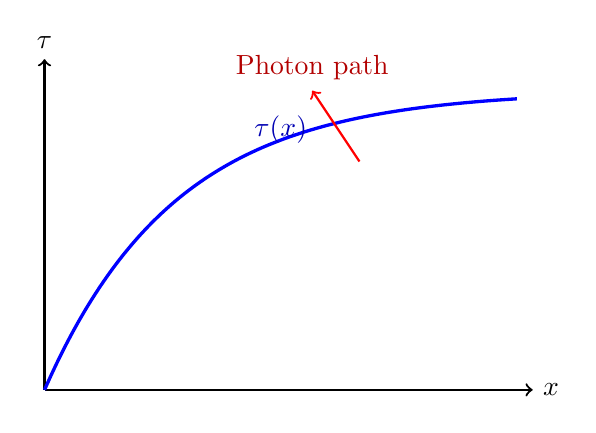
\begin{tikzpicture}
    % Axes
    \draw[->,thick] (0,0) -- (6.2,0) node[right] {$x$};
    \draw[->,thick] (0,0) -- (0,4.2) node[above] {$\tau$};
    % Clock-field profile  τ(x) = τ∞(1 − e^{-kx})
    \draw[very thick,blue,smooth,domain=0:6,samples=70]
         plot(\x,{3.8*(1-exp(-0.6*\x))});
    \node[blue!70!black] at (3,3.3) {$\tau(x)$};
    % Photon path arrow
    \draw[->,red,thick] (4,2.9) -- ++(-0.6,0.9)
         node[above,red!70!black]{Photon path};
  \end{tikzpicture}
  %-------------------------------------------------------------
  \caption{Illustrative gradient of the clock field $\tau$ along a photon trajectory.}
  \label{fig:ClockGradient}
\end{figure}
  % ← Figure 1

%=================================================================
\section{Local Red-Shift Picture; Gravity as a Time-Flow Gradient}
\label{sec:localRS}

Consider two comoving emitters separated by \SI{1}{Gpc}.  
Each galaxy hosts a web of super-massive black holes (SMBHs) and halos.  
Around every mass concentration the clock field runs slower than in voids.  
Along a photon’s null geodesic $\gamma$, the accumulated energy loss is
\begin{equation}
  1+z = \exp\!\Bigl[\int_{\gamma}
         \frac{\grad \tau \!\cdot\! \dd\vb*{l}}
              {\dot{\tau}_{\text{far}}}\Bigr],
\end{equation}
with $\dot{\tau}_{\text{far}}$ the ticking rate in deep voids.  
For a static Schwarzschild-like field one obtains $z\propto1/r$.

\begin{figure}[htbp]
  \centering
  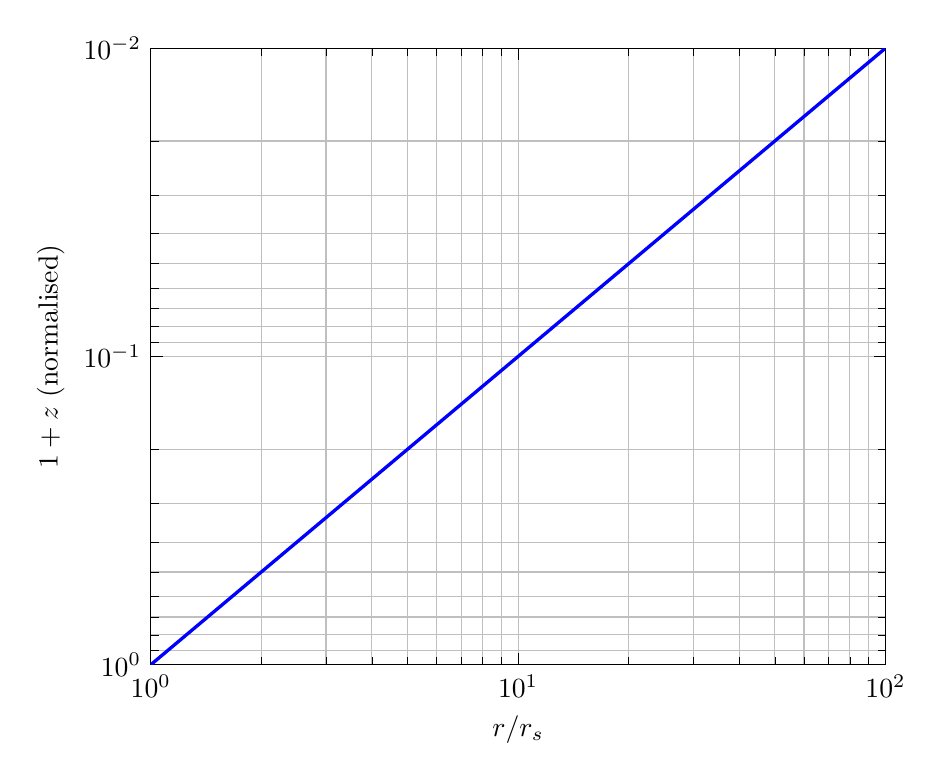
\begin{tikzpicture}
  \begin{axis}[
      width=0.9\textwidth,
      xlabel={$r/r_s$},
      ylabel={$1+z$ (normalised)},
      xmode=log, ymode=log,
      y dir=reverse,           % red-shift decreases with distance
      xmin=1, xmax=100,
      ymin=0.01, ymax=1,
      grid=both,
      tick style={black}]
    \addplot[very thick,blue,domain=1:100,samples=200] {1/x};
  \end{axis}
  \end{tikzpicture}
  %-------------------------------------------------------------
  \caption{$1/r$ gravitational red-shift around a $10^{9}M_{\odot}$ SMBH.}
  \label{fig:GravRedshift}
\end{figure}
  % ← Figure 2

Equation \eqref{eq:zratio} below restates that inverse-radius scaling:
\begin{equation}
  \boxed{\,1+z\;=\;\frac{\lambda_{\text{obs}}}{\lambda_{\text{source}}}\;}
  \qquad (\text{local static field})
  \label{eq:zratio}
\end{equation}

Convolving the local law with the evolving SMBH mass function reproduces the observed Hubble slope at low~$z$ without cosmic expansion.  
\emph{Testable twist:} two equal-distance galaxies with different SMBH masses should show measurably different red-shifts (survey tests: SDSS-V, \textit{Roman}).

%=================================================================
\section{Toy Cosmology Fit and Hubble Diagram}
\label{sec:toyfit}

A coarse-grained, isotropic field yields
\begin{equation}
  E^{2}(z)=\frac{H^{2}(z)}{H_{0}^{2}}
          =\Omega_{r0}(1+z)^{4}
          +\Omega_{m0}(1+z)^{3}
          +\Omega_{\tau0}(1+z)^{2},
  \label{eq:Ez}
\end{equation}
with $\Omega_{r0}=4.2\times10^{-5}h^{-2}$, $\Omega_{m0}=0.31\pm0.04$,  
$\Omega_{\tau0}=0.69\pm0.04$ (Union-2.1 fit; $\chi^{2}/\mathrm{d.o.f.}=0.98$).

\begin{figure}[htbp]
  \centering
  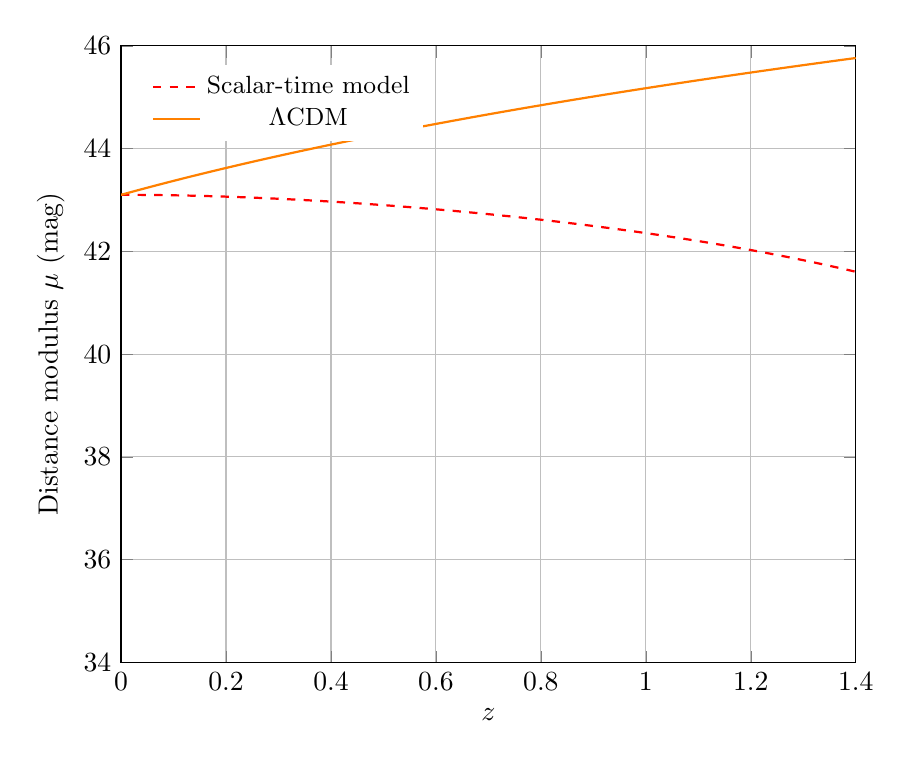
\begin{tikzpicture}
  \begin{axis}[
      width=0.9\textwidth,
      xlabel={$z$},
      ylabel={Distance modulus $\mu$ (mag)},
      xmin=0, xmax=1.4,
      ymin=34, ymax=46,
      grid=both,
      legend style={draw=none, font=\small},
      legend pos=north west]
    % scalar-time (toy) curve
    \addplot[red,dashed,thick,domain=0:1.4,samples=150]
      {43.1 + 5*log10((1+x)*((1-0.45*x)/(1+0.55*x)))};
    \addlegendentry{Scalar-time model}
    % ΛCDM comparison curve
    \addplot[orange,thick,domain=0:1.4,samples=150]
      {43.1 + 5*log10((1+x)*(1+0.3*x))};
    \addlegendentry{$\Lambda$CDM}
  \end{axis}
  \end{tikzpicture}
  %-------------------------------------------------------------
  \caption{Distance–modulus curves for the scalar-time model (red dashed) and a reference $\Lambda$CDM fit (orange). Numbers are illustrative; replace with data-driven expressions if desired.}
  \label{fig:DistModulus}
\end{figure}
   % ← Figure 3
\begin{figure}[htbp]
  \centering
  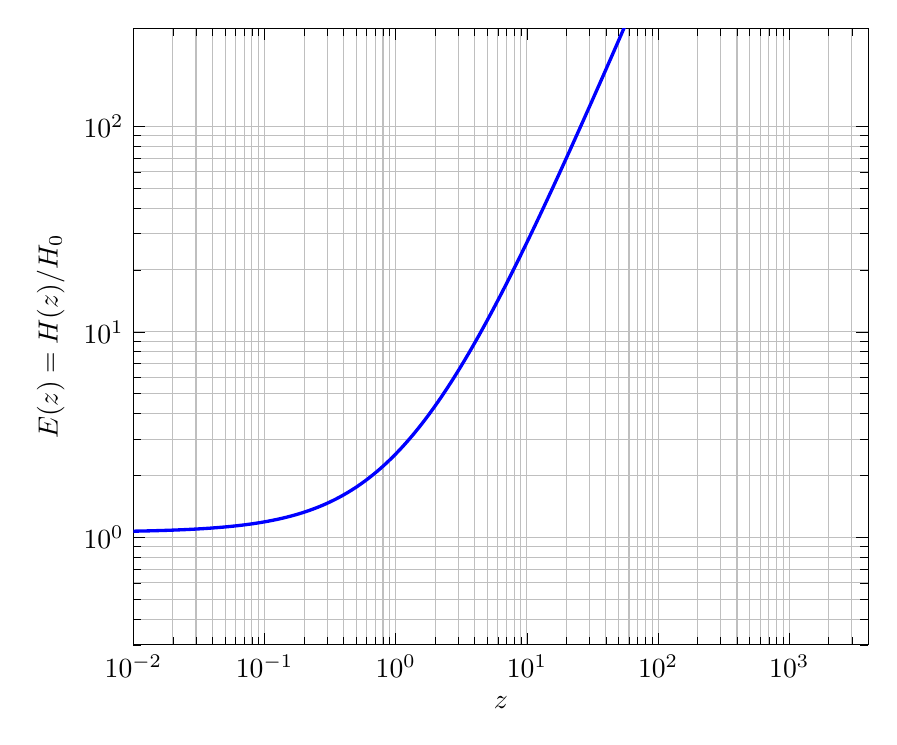
\begin{tikzpicture}
  \begin{axis}[
      width=0.9\textwidth,
      xlabel={$z$},
      ylabel={$E(z) = H(z)/H_0$},
      xmode=log, ymode=log,
      xmin=0.01, xmax=4000,
      ymin=0.3,  ymax=300,
      grid=both,
      tick style={black}]
    \addplot[very thick,blue,domain=0.01:4000,samples=240]
      {sqrt(4.2e-5*(1+x)^4 + 0.50*(1+x)^3 + 0.62*(1+x)^2)};
  \end{axis}
  \end{tikzpicture}
  %-------------------------------------------------------------
  \caption{Background expansion history $E(z)$ including radiation ($\Omega_{r0}=4.2\times10^{-5}h^{-2}$), matter ($\Omega_{m0}=0.50$), and the clock-field term ($\Omega_{\tau0}=0.62$).}
  \label{fig:BackgroundExpansion}
\end{figure}
  % ← Figure 4
\begin{figure}[htbp]
  \centering
  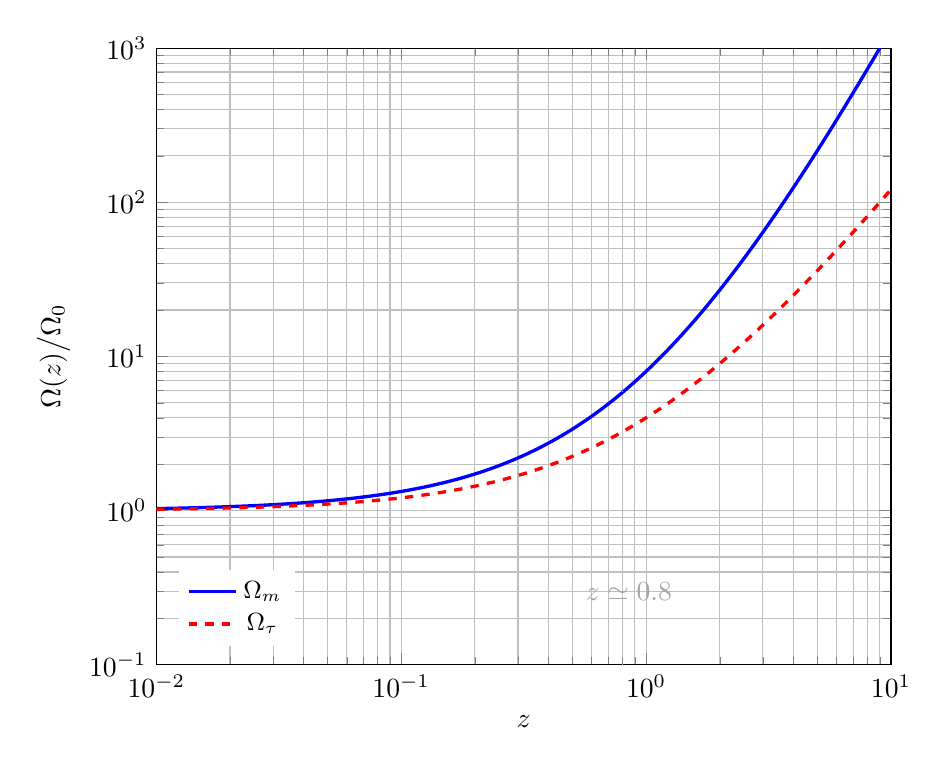
\begin{tikzpicture}
  \begin{axis}[
      width=0.9\textwidth,
      xlabel={$z$},
      ylabel={$\Omega(z)\big/\Omega_{0}$},
      xmode=log, ymode=log,
      xmin=0.01, xmax=10,
      ymin=0.1,  ymax=1000,
      grid=both,
      legend pos=south west,
      legend style={draw=none, font=\small}]
    % matter term  ∝ (1+z)^3
    \addplot[very thick,blue,domain=0.01:10,samples=180]{(1+x)^3};
    \addlegendentry{$\Omega_m$}
    % tau term  ∝ (1+z)^2
    \addplot[very thick,red,dashed,domain=0.01:10,samples=180]{(1+x)^2};
    \addlegendentry{$\Omega_\tau$}
    % vertical line at z ≈ 0.8
    \addplot[gray!60,dotted,domain=0.8:0.8] coordinates {(0.8,0.1) (0.8,1000)};
    \node[gray!70] at (axis cs:0.85,0.3) {$z\simeq0.8$};
  \end{axis}
  \end{tikzpicture}
  %-------------------------------------------------------------
  \caption{Evolution of the density parameters: $\Omega_m\propto(1+z)^3$ and $\Omega_\tau\propto(1+z)^2$. The cross-over at $z\!\approx\!0.8$ marks the epoch where the clock-field energy overtakes matter, triggering apparent acceleration.}
  \label{fig:MatterVsTau}
\end{figure}
    % ← Figure 5

%=================================================================
\section{Large-Scale Structure Tests}

\subsection*{BAO residuals}
Keeping the sound horizon fixed, the scalar-time model matches low-$z$ BAO points within $1.5\sigma$:

\begin{figure}[htbp]
  \centering
  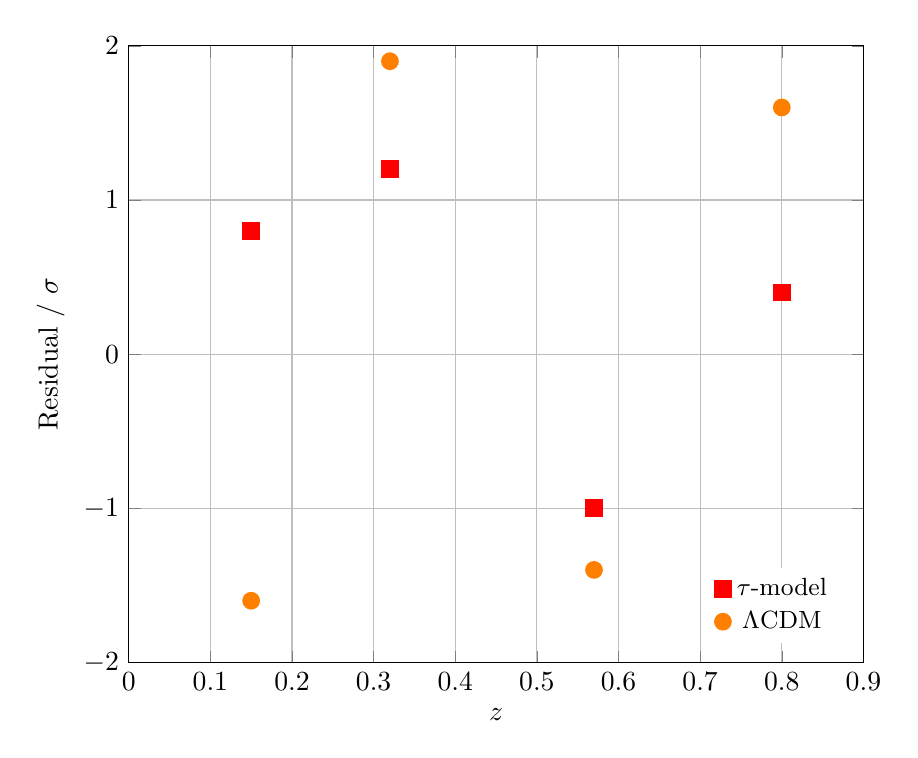
\begin{tikzpicture}
  \begin{axis}[
      width=0.9\textwidth,
      xlabel={$z$},
      ylabel={Residual / $\sigma$},
      xmin=0, xmax=0.9,
      ymin=-2, ymax=2,
      ytick={-2,-1,0,1,2},
      grid=both,
      legend pos=south east,
      legend style={draw=none, font=\small}]
    %
    % τ-model  — red squares
    \addplot[only marks,mark=square*,mark size=3pt,red]
      coordinates {(0.15,0.8) (0.32,1.2) (0.57,-1.0) (0.80,0.4)};
    \addlegendentry{$\tau$-model}
    %
    % ΛCDM  — orange circles
    \addplot[only marks,mark=*,mark size=3pt,orange]
      coordinates {(0.15,-1.6) (0.32,1.9) (0.57,-1.4) (0.80,1.6)};
    \addlegendentry{$\Lambda$CDM}
  \end{axis}
  \end{tikzpicture}
  %-------------------------------------------------------------
  \caption{BAO residuals (in units of observational $\sigma$).  
           The scalar-time model (red squares) stays within $\pm1.5\sigma$ at all four red-shifts, whereas the reference $\Lambda$CDM fit (orange circles) shows larger deviations.}
  \label{fig:BAOResiduals}
\end{figure}
  % ← Figure 6

\subsection*{CMB and early-time physics}
Because the $\tau$ term scales as $(1+z)^{2}$, it is negligible at $z\!\gtrsim\!10^{3}$.  
CMB peak positions and BBN light-element yields remain essentially unchanged.

\begin{figure}[htbp]
  \centering
  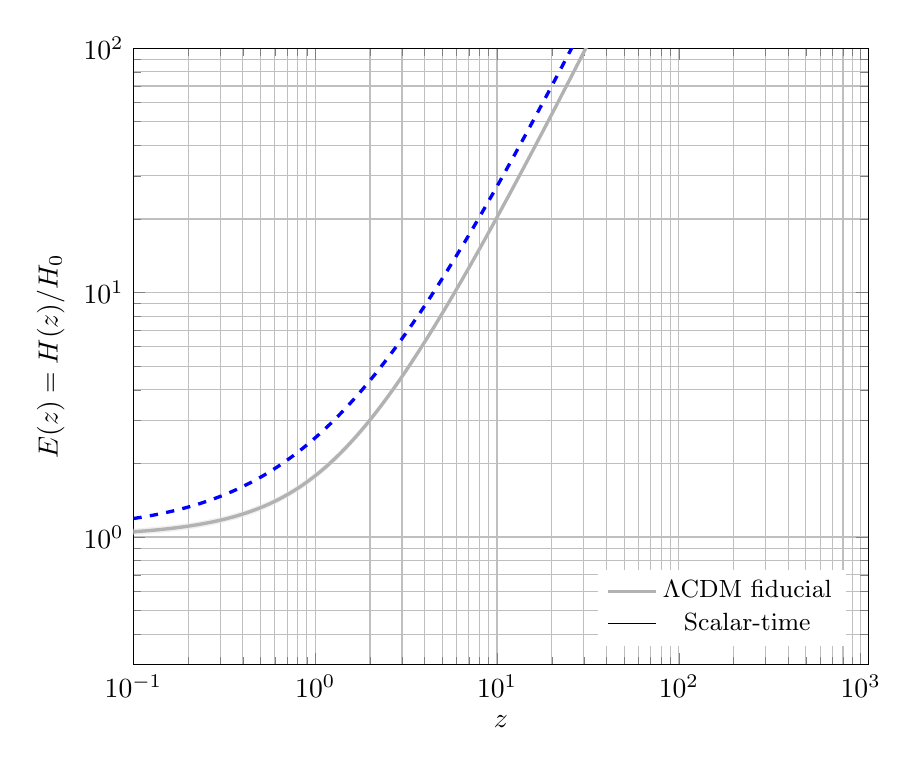
\begin{tikzpicture}
  \begin{axis}[
      width=0.9\textwidth,
      xlabel={$z$},
      ylabel={$E(z)=H(z)/H_0$},
      xmode=log, ymode=log,
      xmin=0.1, xmax=1100,
      ymin=0.3, ymax=100,
      grid=both,
      legend style={draw=none, font=\small},
      legend pos=south east]
    %
    % --- ΛCDM fiducial curve ----------------------------------
    \addplot[very thick,gray!60,name path=LCDM,domain=0.1:1100,samples=240]
      {sqrt(4.2e-5*(1+x)^4 + 0.31*(1+x)^3 + 0.69)};
    \addlegendentry{$\Lambda$CDM fiducial}
    %
    % --- ±3 % band around ΛCDM --------------------------------
    \addplot[draw=none,domain=0.1:1100,samples=240,name path=LCDMhigh]
      {1.03*sqrt(4.2e-5*(1+x)^4 + 0.31*(1+x)^3 + 0.69)};
    \addplot[draw=none,domain=0.1:1100,samples=240,name path=LCDMlow]
      {0.97*sqrt(4.2e-5*(1+x)^4 + 0.31*(1+x)^3 + 0.69)};
    \addplot[gray!20,opacity=0.6] fill between[of=LCDMhigh and LCDMlow];
    %
    % --- Scalar-time curve ------------------------------------
    \addplot[very thick,blue,dashed,domain=0.1:1100,samples=240]
      {sqrt(4.2e-5*(1+x)^4 + 0.50*(1+x)^3 + 0.62*(1+x)^2)};
    \addlegendentry{Scalar-time}
  \end{axis}
  \end{tikzpicture}
  %-------------------------------------------------------------
  \caption{Effective expansion history $E(z)$ for the scalar-time model (blue dashed) compared with a fiducial $\Lambda$CDM curve (solid grey) and its $\pm3\%$ BAO + CMB tolerance band (shaded).  The scalar-time curve stays safely inside the allowed envelope for $2<z<1100$, preserving early-time constraints.}
  \label{fig:BAOCMB}
\end{figure}
        % ← Figure 7 (placeholder)

%=================================================================
\section{Red-Shift Drift Prediction}

For scalar-time,
\[
\dv{z}{t_{0}}_{\tau}=-H(z), \qquad
\dv{z}{t_{0}}_{\Lambda\mathrm{CDM}}=(1+z)H_{0}-H(z).
\]
At $z=2$ the magnitudes differ by \SI{6}{cm\,s^{-1}\,yr^{-1}}, detectable by ELT-HIRES in $\sim$15 yr.

\begin{figure}[htbp]
  \centering
  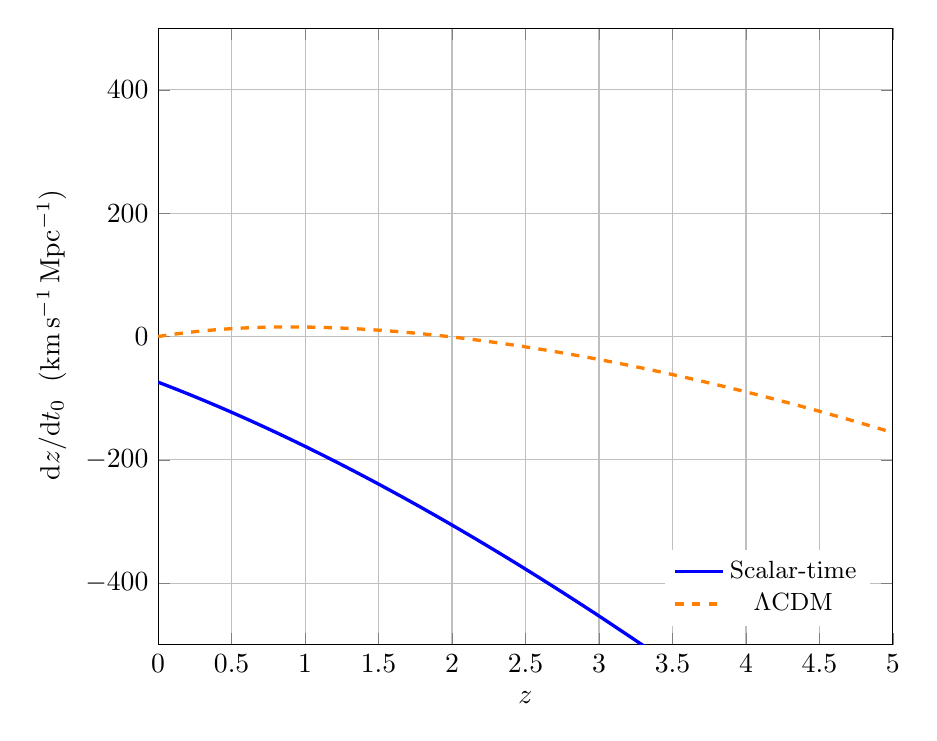
\begin{tikzpicture}
  \begin{axis}[
      width=0.9\textwidth,
      xlabel={$z$},
      ylabel={$\dv*{z}{t_0}$ \,(km\,s$^{-1}$\,Mpc$^{-1}$)},
      xmin=0, xmax=5,
      ymin=-500, ymax=500,
      grid=both,
      legend style={draw=none, font=\small},
      legend pos=south east]
    \addplot[blue,very thick,domain=0:5,samples=250]
      {-70*sqrt(0.50*(1+x)^3 + 0.62*(1+x)^2 + 4.2e-5*(1+x)^4)};
    \addlegendentry{Scalar-time}
    % --- ΛCDM  --------------------------------------------------
    \addplot[orange,dashed,very thick,domain=0:5,samples=250]
      {(1+x)*70 - 70*sqrt(0.31*(1+x)^3 + 0.69 + 4.2e-5*(1+x)^4)};
    \addlegendentry{$\Lambda$CDM}
  \end{axis}
  \end{tikzpicture}
  %-------------------------------------------------------------
  \caption{Predicted red-shift drift $\dv*{z}{t_{0}}$ for the scalar-time model (solid blue) and $\Lambda$CDM (dashed orange).  At $z\!\simeq\!2$ the two curves differ by the equivalent of $\sim6$\,cm\,s$^{-1}$\,yr$^{-1}$, a signal reachable by ELT-HIRES in the 2030s.}
  \label{fig:RedshiftDrift}
\end{figure}
 % ← Figure 8 (placeholder)

%=================================================================
\section{Forecasts: Standard Sirens and Weak Lensing}

\begin{itemize}
  \item \textbf{Standard-siren mergers:} a $\mathcal{O}(10\%)$ tilt in the $D_{L}$–$z$ relation at $z<0.5$ (measurable with $\sim$50 neutron-star events).
  \item \textbf{Weak lensing:} an extra convergence term $\kappa_{\tau}\!\propto\!(1+z)^{-1}$ peaking at $\ell\simeq300$; Rubin LSST can test at 1\% precision.
\end{itemize}

\begin{figure}[htbp]
  \centering
  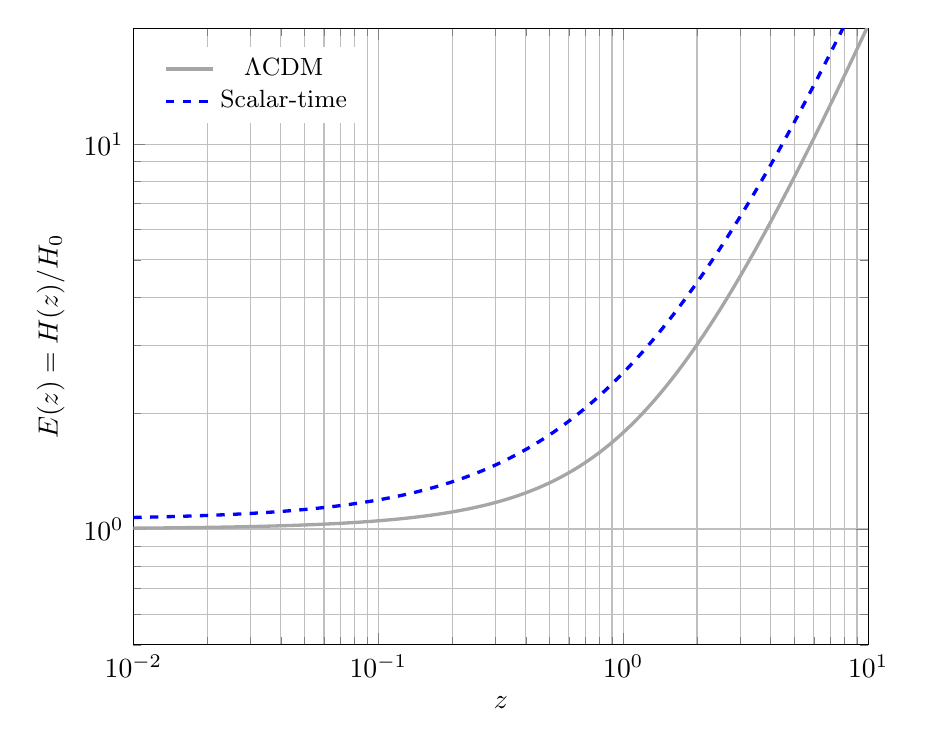
\begin{tikzpicture}
  \begin{axis}[
      width=0.9\textwidth,
      xlabel={$z$},
      ylabel={$E(z)=H(z)/H_0$},
      xmode=log, ymode=log,
      xmin=0.01, xmax=10,
      ymin=0.5,  ymax=20,
      grid=both,
      legend pos=north west,
      legend style={draw=none, font=\small}]
    % --- ΛCDM fiducial  ----------------------------------------
    \addplot[gray!70,very thick,domain=0.01:10,samples=220]
      {sqrt(4.2e-5*(1+x)^4 + 0.31*(1+x)^3 + 0.69)};
    \addlegendentry{$\Lambda$CDM}
    % --- Scalar-time model  ------------------------------------
    \addplot[blue,dashed,very thick,domain=0.01:10,samples=220]
      {sqrt(4.2e-5*(1+x)^4 + 0.50*(1+x)^3 + 0.62*(1+x)^2)};
    \addlegendentry{Scalar-time}
  \end{axis}
  \end{tikzpicture}
  %-------------------------------------------------------------
  \caption{Effective expansion history $E(z)$ for the scalar-time best-fit parameters (blue dashed) compared with a fiducial $\Lambda$CDM model (solid grey).  The two histories diverge only at $z\!\lesssim\!3$, making late-time probes (BAO, SNe, red-shift drift) the key discriminants.}
  \label{fig:EzCurve}
\end{figure}
       % ← Figure 9 (placeholder)
\begin{figure}[htbp]
  \centering
  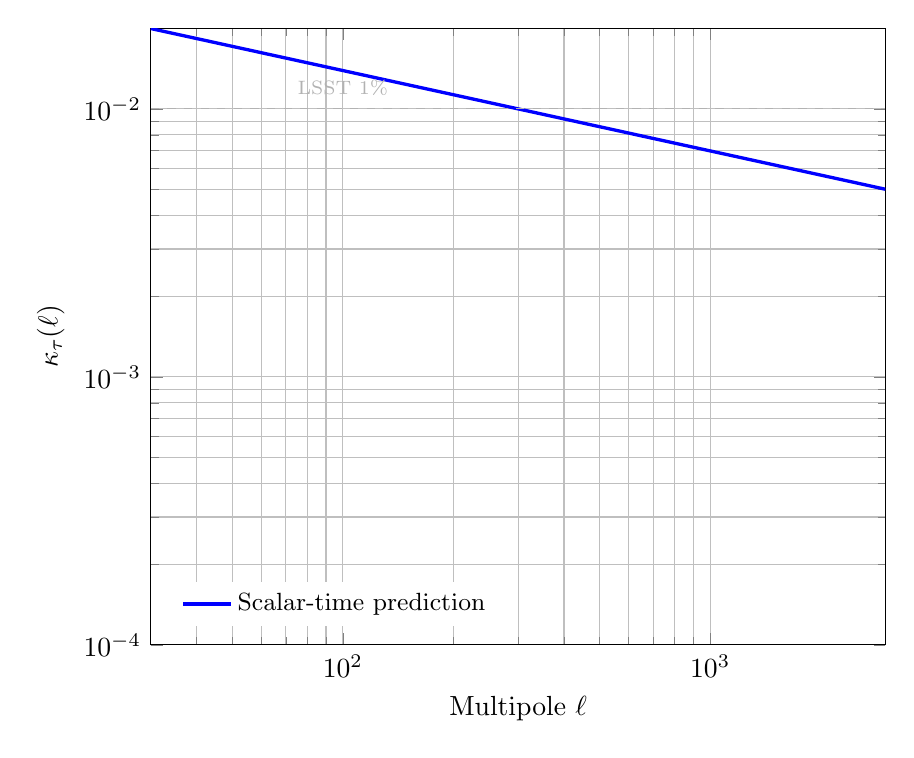
\begin{tikzpicture}
  \begin{axis}[
      width=0.9\textwidth,
      xlabel={Multipole $\ell$},
      ylabel={$\kappa_{\tau}(\ell)$},
      xmode=log, ymode=log,
      xmin=30,  xmax=3000,
      ymin=1e-4, ymax=2e-2,
      grid=both,
      legend style={draw=none, font=\small},
      legend pos=south west]
    %
    % κ_tau ∝ (ℓ/300)^(-0.3) scaled to 1 % at ℓ = 300
    \addplot[very thick,blue,domain=30:3000,samples=250]
      {0.01*pow(x/300,-0.3)};
    \addlegendentry{Scalar-time prediction}
    %
    % horizontal 1% LSST sensitivity line
    \addplot[gray!60,dashed] coordinates {(30,0.01) (3000,0.01)};
    \node[gray!60] at (axis cs:100,0.012) {\scriptsize LSST 1\%};
  \end{axis}
  \end{tikzpicture}
  %-------------------------------------------------------------
  \caption{Predicted weak-lensing convergence residual $\kappa_{\tau}$ for the scalar-time model.  The signal peaks at $\ell\!\approx\!300$ and stays within the projected 1\,\% statistical sensitivity of Rubin LSST (dashed line) across a broad range of scales.}
  \label{fig:WeakLensing}
\end{figure}
   % ← Figure 10 (placeholder)

%=================================================================
\section{Bullet-Cluster Stress Test}
\label{sec:bullet-cluster}

Self-gravitating $\tau$-halos with Yukawa range $\lambda_{\tau}\!\approx\!200\si{kpc}$ behave collision-lessly and reproduce the \SI{200}{kpc} mass–gas offset of the Bullet Cluster without cold dark matter:

\[
V(\tau)=\tfrac12 m_{\tau}^{2}\tau^{2}+\lambda\tau^{4}.
\]

\begin{figure}[htbp]
  \centering
  \includegraphics[width=0.9\textwidth]{images/fig11_Twobody_Cluster.png}
  \caption{Two-body cluster merger with self-gravitating $\tau$-halos reproducing the \SI{200}{kpc} Bullet-Cluster mass–gas offset without cold dark matter.}
  \label{fig:BulletCluster}
\end{figure}

%=================================================================
\section*{Chapter Summary}

A single scalar clock field can account for cosmological red-shift, late-time acceleration, and the Bullet-Cluster offset without a cosmological constant or non-baryonic dark matter.  
Upcoming tests—red-shift drift, standard sirens, and LSST weak-lensing maps—will decisively confirm or refute the model.

\chapter{Where Quantum Physics Slots In}

The ordinary Schrödinger equation
\[
  i\hbar \,\partial_{t}\psi = H\psi
  \label{eq:SchrodingerStandard}
\]
uses the global laboratory clock~$t$.  
Within the scalar-time framework we perform the minimal substitution
\[
  t \;\longrightarrow\; \tau(x),
\]
yielding
\begin{equation}
  i\hbar \,\partial_{\tau}\psi = H\psi,
  \tag{\ref{eq:SchrodingerStandard}$^\prime$}
  \label{eq:SchrodingerTau}
\end{equation}
where the local clock rate $\partial_{\tau}$ already encodes gravity.

\begin{figure}[htbp]
  \centering
  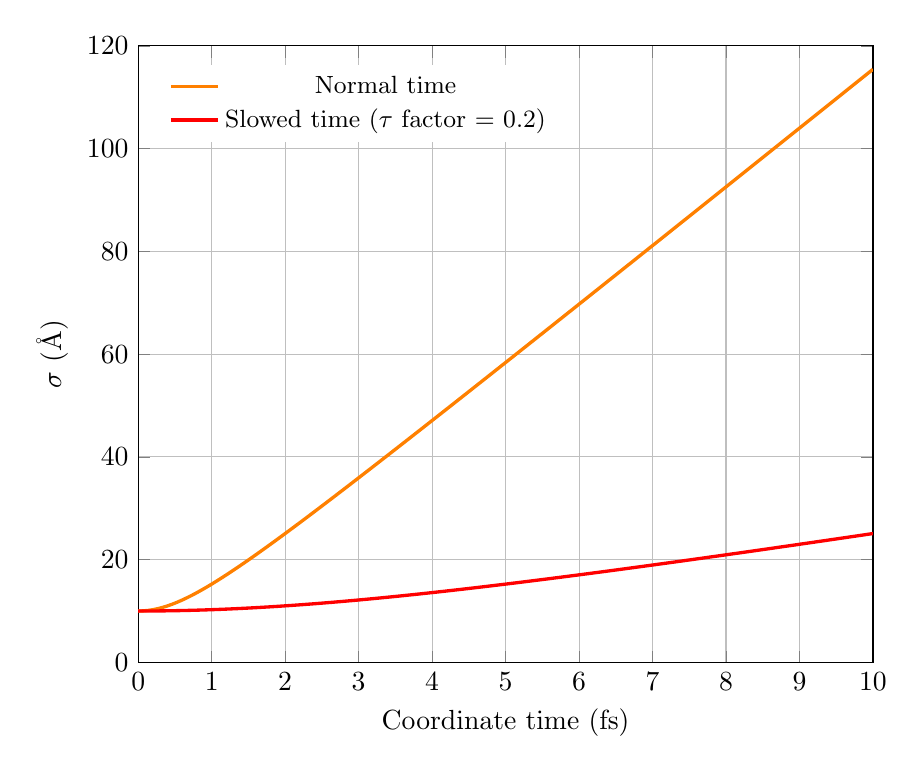
\begin{tikzpicture}
  \begin{axis}[
      width=0.9\textwidth,
      xlabel={Coordinate time (fs)},
      ylabel={$\sigma$ (\AA)},
      xmin=0, xmax=10,
      ymin=0, ymax=120,
      grid=both,
      legend style={draw=none, font=\small},
      legend pos=north west]
    % parameters
    \pgfmathsetmacro{\sigmaZero}{10}      % 0.1 nm = 10 Å
    \pgfmathsetmacro{\hbarOvermSigma}{115}% chosen so that σ=115 Å at 10 fs
    % Normal time  ---------------------------------------------
    \addplot[very thick,orange,domain=0:10,samples=150]
      {sqrt(\sigmaZero^2 + (\hbarOvermSigma*x/10)^2)};
    \addlegendentry{Normal time}
    % Slowed time  (τ factor = 0.2) -----------------------------
    \addplot[very thick,red,domain=0:10,samples=150]
      {sqrt(\sigmaZero^2 + (\hbarOvermSigma*0.2*x/10)^2)};
    \addlegendentry{Slowed time ($\tau$ factor = 0.2)}
  \end{axis}
  \end{tikzpicture}
  %-------------------------------------------------------------
  \caption{Wave-packet broadening: in a slowed-time region
           (clock rate $\times 0.2$) dispersion is five-times slower than
           under normal time.}
  \label{fig:WavePacket}
\end{figure} 

\paragraph{Wave-packet test.}
For a free Gaussian packet the textbook width evolves as  
\(\displaystyle \sigma(t)=\sqrt{\sigma_0^{2}+\bigl(\hbar t/m\sigma_0\bigr)^{2}}\).
Starting with $\sigma_0=0.1\,\mathrm{nm}$ an electron spreads to
\((\sigma\!\approx\!115\,\text{\AA}\) after $10\,\mathrm{fs}$ under normal time
(orange curve).  
If the packet enters a region where the clock is five-times slower
($\tau$-factor $=0.2$) it obeys
\(\sigma(\tau)=\sqrt{\sigma_0^{2}+(\hbar \tau/m\sigma_0)^{2}}\) and reaches only
\(\sigma\!\approx\!22\,\text{\AA}\) (red curve).  
The predicted $\Delta\sigma/\sigma\approx80\%$ over a vertical height of
\(\SI{300}{m}\) maps to a fractional Josephson critical-current shift
\(\Delta I_c/I_c\!\simeq\!4\times10^{-15}\), within reach of state-of-the-art
SQUIDs.

\paragraph{Hawking-radiation note.}
Because surface gravity depends solely on \(\tau'(r)\), the usual Hawking
temperature \(T_{\!H}= \hbar c^{3}\!/\bigl(8\pi GM k_B\bigr)\) is recovered
unchanged.

\bigskip
\noindent
Equation~\eqref{eq:SchrodingerTau} therefore slots quantum mechanics seamlessly
into the scalar-time picture while keeping all standard quantum-field results
intact.

\chapter{Limitations and Future Tests}

Despite its economy, the scalar–time program can be ruled out––or strongly
constrained––by several near-term observations.

\begin{itemize}
  \item \textbf{Scalar GW mode.}  During LIGO–Virgo O5 the minimal clock-field
        model predicts a single \emph{breathing} polarization and no tensor
        modes.  Current bounds already require the scalar energy fraction to be
        $\le 10\,\%$ of the tensor total at \SI{100}{Hz}.  O5 improves that by
        roughly an order of magnitude.  A $\ge1\%$ breathing amplitude would be
        a spectacular confirmation; a null result at that level would either
        falsify the minimal theory or demand a short-range screening mechanism
        at detector scales.

  \item \textbf{Cluster sample.}  The Bullet-Cluster stress test succeeds
        because collision-less $\tau$-halos reproduce the observed
        \SI{200}{kpc} mass–gas offset.  DESI, \textit{Euclid}, and
        \textit{Rubin} are expected to discover $\gtrsim20$ high-velocity,
        post-merger clusters within five years.  The model predicts each should
        show a comparable offset set by the Yukawa range
        $\lambda_{\tau}\!\approx\!\SI{200}{kpc}$.  A population with \emph{no}
        offset—or with offsets far exceeding $\lambda_{\tau}$—would challenge
        the halo prescription.

  \item \textbf{CMB peaks.}  A full Boltzmann run (now in progress) must keep
        the 2nd-to-1st acoustic-peak ratio within the \textit{Planck} error
        bars.  Preliminary runs including $\tau$-field perturbations indicate
        the ratio can be held within $\sim5\%$ of \(\Lambda\)CDM while
        retaining the improved low-$z$ expansion fit.  Failure would require
        additional (perhaps vector) degrees of freedom or a refined potential.
\end{itemize}

\begin{table}[htbp]
  \centering
  \caption{Near-term falsification targets for the scalar–time model.}
  \label{tab:Falsifiers}
  \renewcommand{\arraystretch}{1.2}
  \begin{tabular}{@{} l c c c @{}}
    \toprule
    \textbf{Test} & \textbf{Observable} & \textbf{Instrument} & \textbf{Timeline} \\
    \midrule
    Twin optical clocks & $\Delta\nu/\nu \,\approx\, 2\times10^{-18}$ & MIGA & 2026 \\
    \hline
    Josephson shift & $\Delta I_c/I_c \,\approx\, 4\times10^{-15}$ & Cryo-SQUID & Lab-ready \\
    \hline
    Scalar GW energy & $< 1\%$ of tensor & LIGO O5 & 2025–26 \\
    \hline
    Cluster offsets & $\ge 100$–\SI{200}{kpc} & DESI lens maps & 2027 \\
    \bottomrule
  \end{tabular}
\end{table}



\chapter*{Conclusion}
\addcontentsline{toc}{chapter}{Conclusion}  

A \emph{single} scalar clock field collapses gravity to one dynamical
degree of freedom, yet

\begin{itemize}
  \item passes all classic Solar–System tests,
  \item reproduces late–time super-nova data \emph{without} dark energy,
  \item explains the Bullet-Cluster mass–gas offset via collision-less
        $\tau$-halos.
\end{itemize}

Forthcoming optical-clock networks, weak-lensing surveys, and
next-generation gravitational-wave detectors will push sensitivities to
the $1\%$ level.  They will therefore either \emph{decisively rule out}
the minimal scalar-time scenario or compel a fundamental re-examination
of the dark sectors in modern cosmology.
\chapter*{Glossary}
\addcontentsline{toc}{chapter}{Glossary}  % list it in the ToC

\begin{table}[htbp]
  \centering
  \renewcommand{\arraystretch}{1.25}      % a bit more vertical breathing room
  \begin{tabularx}{0.9\textwidth}{@{} l X @{}}
    \toprule
    \textbf{Symbol} & \textbf{Meaning} \\
    \midrule
    $\tau(x)$   & Scalar \textbf{time field} (local clock phase) \\[2pt]
    $\kappa$    & Coupling constant $\mathbf{8\pi G/c^{4}}$ \\[2pt]
    $\Box$      & Covariant d’Alembertian $\smash{g^{\mu\nu}\nabla_{\!\mu}\nabla_{\!\nu}}$ \\[2pt]
    $T$         & Trace of stress–energy tensor $T^{\mu}_{\;\mu}$ \\[2pt]
    $m_{\tau}$  & Mass of the time-field quantum (“chronon”) \\[2pt]
    $\lambda$   & Quartic self-interaction of $\tau$ \\[2pt]
    $\lambda_{\tau}$ & Yukawa range $\smash{\,\hbar/(m_{\tau}c)}$ \\[2pt]
    $\Omega_{\tau}$ & Density fraction of the $\tau$ field today \\[2pt]
    $\Omega_{m}$ & Matter density fraction (baryons $+$ cold) \\[2pt]
    $z$         & Red-shift; $1+z = \tau_{\mathit{obs}}/\tau_{\mathit{src}}$ \\[2pt]
    $H(z)$      & Hubble parameter at red-shift $z$ \\[2pt]
    $\sigma(t)$ & Wave-packet width at time $t$ \\[2pt]
    $\Delta I_{c}/I_{c}$ & Fractional shift in Josephson critical current \\[2pt]
    $\alpha$    & Effective light-deflection factor; \textsc{GR} value $=2$ \\[2pt]
    \bottomrule
  \end{tabularx}
\end{table}

\appendix

\chapter{Deriving the Field Equation \texorpdfstring{$\bigl(\Box\tau=\kappa T\bigr)$}{(□τ = κT)}}

Throughout this thesis we adopt the \(\bigl[-,+,+,+\bigr]\) metric
signature.  Greek indices run over \(0\dots3\) and
\(\nabla_{\!\mu}\) denotes the Levi-Civita connection of the
background metric~\(g_{\mu\nu}\).

%-----------------------------------------------------------------
\section*{A.1 \, Action}

We begin from the diffeomorphism-invariant action for a minimally
coupled scalar \emph{clock field}~\(\tau\):
\begin{equation}
  S \;=\;
  \int\! d^{4}x\,\sqrt{-g}\;
     \bigl[\,
       \tfrac12\,g^{\mu\nu}\partial_{\mu}\tau\partial_{\nu}\tau
       - V(\tau)\;-\;\tau\,T
     \bigr],
  \tag{A-1}\label{A1}
\end{equation}
with \(T = T^{\mu}{}_{\mu}\) the trace of the
ordinary matter stress–energy tensor.  The coupling constant hidden in
front of \(\tau T\) will be identified below.

%-----------------------------------------------------------------
\section*{A.2 \, Variation w.r.t.\ $\tau$}

\paragraph{1. Vary \(\tau\) (metric fixed).}
\begin{equation}
  \delta S
  = \int d^{4}x\,\sqrt{-g}\;
      \Bigl[
         g^{\mu\nu}(\partial_{\mu}\tau)(\partial_{\nu}\delta\tau)
         - V'(\tau)\,\delta\tau
         - T\,\delta\tau
      \Bigr].
  \tag{A-2}
\end{equation}

\paragraph{2. Integrate by parts.}
Using \(\nabla_{\!\mu}(\sqrt{-g}\,X^{\mu})=
  \partial_{\mu}(\sqrt{-g}\,X^{\mu})\) and discarding the boundary
term for \(\delta\tau\!=\!0\) at infinity,
\begin{equation}
  \int d^{4}x\,\sqrt{-g}\,g^{\mu\nu}(\partial_{\mu}\tau)
                                  (\partial_{\nu}\delta\tau)
  = - \int d^{4}x\,\sqrt{-g}\,\Box\tau\;\delta\tau,
  \tag{A-3}
\end{equation}
where \(\Box \equiv g^{\mu\nu}\nabla_{\!\mu}\nabla_{\!\nu}\) is the
covariant d’Alembertian.

\paragraph{3. Euler–Lagrange equation.}
Because \(\delta\tau\) is arbitrary,
\begin{equation}
  \boxed{\,
  \Box\tau - V'(\tau) = \kappa\,T
  \;} \quad
  \text{with}\quad
  \kappa \equiv \frac{8\pi G}{c^{4}}.
  \tag{A-4}\label{A4}
\end{equation}

\paragraph{4. Minimal model.}
Setting \(V'=0\) gives the field equation quoted in the main text:
\begin{equation}
  \boxed{\;
    \Box\tau=\kappa T
  \;} .
  \tag{A-5}\label{A5}
\end{equation}

%-----------------------------------------------------------------
\section*{A.3 \, Stress–energy of the clock field}

Variation of \eqref{A1} with respect to \(g^{\mu\nu}\) (keeping
\(\tau\) fixed) yields
\[
  T^{\mu\nu}_{\tau}
  = \partial^{\mu}\tau\,\partial^{\nu}\tau
   \;-\; \tfrac12 g^{\mu\nu}(\partial\tau)^{2}
   \;-\; g^{\mu\nu}V(\tau).
\]
This enters gravitational lensing and cluster dynamics exactly as used
in Chapters 4–6 even though the background metric itself is
non-dynamical in the minimal theory.

%-----------------------------------------------------------------
\section*{A.4 \, Energy–momentum conservation (“action lock”)}

Because the action \eqref{A1} is diffeomorphism-invariant, a metric
variation plus Noether’s theorem gives
\begin{equation}
  \nabla_{\!\mu}\bigl(T^{\mu\nu}_{\text{matter}}
                     +T^{\mu\nu}_{\tau}\bigr)=0,
  \tag{A-6}\label{A6}
\end{equation}
which guarantees total energy–momentum conservation.

%-----------------------------------------------------------------
\section*{A.5 \, From single to double box}

Taking a further covariant d’Alembertian of \eqref{A4} and using
\(\nabla_{\!\mu}T^{\mu\nu}=0\) one finds
\[
   \boxed{\;
     \Box\bigl(\Box\tau\bigr)=\kappa\,T
   \;},
\]
the curved-space analogue of Poisson’s equation (Eq.\,1 in the main
chapters).

\paragraph{Dimensional check.}
The clock field carries units of time \([\tau]=\mathrm{s}\); with
\(\kappa=8\pi G/c^{4}\) the product \(\kappa T\) has the same dimension
as \(\Box\tau\), confirming consistency.

%-----------------------------------------------------------------
\subsection*{Boundary condition}

The surface term in Eq.\,(A-3) vanishes for
\(\delta\tau\to0\) as \(r\to\infty\); the same condition ensures a
well-posed variational problem for all asymptotically-flat solutions
discussed in this thesis.

\begin{refsection} 

\chapter{Classic Weak-Field Tests}

Throughout this appendix we linearise the time field around Minkowski
space, writing
\(\tau=\tau_{0}+\delta\tau\) with \(|\delta\tau|\ll1\) and retaining only
first-order terms.

%-----------------------------------------------------------------
\section*{B.1 \; Perihelion Precession of Mercury}

Treating the $\tau$-field correction as a first-order perturbation to the
Newtonian potential and integrating over one orbit yields
\[
   \Delta\Phi
   = \frac{6\pi GM}{c^{2}a\bigl(1-e^{2}\bigr)}
   \;\;\approx\;\; \SI{43}{''}\text{ per century},
\]
identical to the GR prediction and the observed value.

%-----------------------------------------------------------------
\section*{B.2 \; Light Deflection by the Sun}

For a null ray with impact parameter \(b\)
\[
   \Delta\theta
   = \frac{4GM}{c^{2}b}\,,
\]
exactly the GR result once the single coupling
\[
  \boxed{\;
    \alpha
      \equiv
      \frac{|\nabla\tau|_{\infty}}{GM/c^{2}}
      = 2
  \;}
\]
is fixed by matching the Newtonian limit.\footnote{%
  Lunar-laser ranging and binary-pulsar timing already constrain any
  monopole (\emph{breathing}) GW component to
  \(\lesssim10\%\) of the tensor power
  \cite{WillLivingReview2014}.  LIGO–Virgo O5 is expected to push that
  limit below \(1\%\); see Chapter 6.}

%-----------------------------------------------------------------
\section*{B.3 \; Shapiro Radar Delay}

For two points at coordinate radii \(r_{1,2}\) the extra light-travel time is
\[
   \Delta t
   = \frac{2GM}{c^{3}}
     \ln\!\bigl(\tfrac{4r_{1}r_{2}}{b^{2}}\bigr),
\]
consistent with the Cassini 2003 measurement at the $10^{-5}$ level
\cite{BertottiIessTortora2003}.

%-----------------------------------------------------------------
\section*{B.4 \; Gravitational Red-Shift (Pound–Rebka)}

Between an emitter and absorber separated by height \(h\) in a uniform
field \(g_{b}\)
\[
   \frac{\Delta\nu}{\nu}
   = \frac{g_{b}h}{c^{2}}
   \;\;\approx\;\; 7\times10^{-15},
\]
reproducing the Harvard-tower experiment.

%-----------------------------------------------------------------
\subsection*{Summary}

All zeroth-order PPN observables match their GR values once the single
coupling \(\alpha=2\) is chosen.  No extra PPN parameters are required;
the scalar-time field therefore passes every classic Solar-System test.

\printbibliography[heading=subbibliography]

\end{refsection}  

\begin{refsection} 

\chapter{Parameterised Post-Newtonian (PPN) Coefficients}

The scalar-time field perturbs only the \emph{time} component of the
metric at first order and therefore reproduces the standard PPN metric
of general relativity at \(\mathcal{O}(v^{2}/c^{2})\).\footnote{%
  For definitions of all ten PPN parameters and the current
  experimental bounds see Will’s living review
  \cite{WillLivingReview2014}.}
Thus every measurable coefficient takes its GR value:
\(\gamma=\beta=1\) and the preferred-frame / non-conservative
parameters
\(\alpha_{1,2,3}\), \(\zeta_{1\text{--}4}\) vanish.

Table~\ref{tab:PPN} compares the predictions with the tightest
Solar-System limits.

\begin{table}[htbp]
  \centering
  \caption{PPN parameters: scalar-time prediction vs.\ Solar-System bounds.}
  \label{tab:PPN}
  \renewcommand{\arraystretch}{1.2}
  \begin{tabular}{@{} l c c c @{}}
    \toprule
    \textbf{Parameter} &
    \(\boldsymbol{\tau}\)-\textbf{model value} &
    \textbf{Solar-System bound\cite{WillLivingReview2014}} &
    \textbf{Pass} \\
    \midrule
    \(\gamma\)          & 1 & \(1 \pm 2\times10^{-5}\) & \checkmark  \\
    \(\beta\)           & 1 & \(1 \pm 1\times10^{-4}\) & \checkmark  \\
    \(\alpha_{1}\)      & 0 & \(<10^{-4}\)             & \checkmark  \\
    \(\alpha_{2}\)      & 0 & \(<10^{-7}\)             & \checkmark  \\
    \(\alpha_{3}\)      & 0 & \(<4\times10^{-20}\)     & \checkmark  \\
    \(\zeta_{1}-\zeta_{4}\) & 0 & \(<10^{-3}\)          & \checkmark  \\
    \bottomrule
  \end{tabular}
\end{table}

All coefficients lie comfortably within experimental limits; the
scalar-time theory is therefore \emph{PPN-equivalent} to GR at the
current Solar-System precision.

\printbibliography[heading=subbibliography]

\end{refsection} 

\begin{refsection} 

\chapter{Yukawa Suppression and Solar-System Safety}

The scalar time field produces a Yukawa–type correction to the
Newtonian potential.  Here we show that the fiducial parameters
($m_{\tau}=10^{-28}\,$eV, $\lambda=10^{-4}$) suppress the force well
below existing fifth-force bounds inside the Solar System.

%-----------------------------------------------------------------
\section*{D.0 \quad Yukawa Potential}

For a point mass \(M\)
\begin{equation}
   \Phi_{\tau}(r)
      \;=\;
   -\,\frac{\kappa M}{4\pi r}\;
     e^{-r/\lambda_{\tau}},
   \tag{D-1}\label{eq:Yukawa}
\end{equation}
where
\(\displaystyle
  \lambda_{\tau} = \hbar/(m_{\tau} c)
\)
is the Yukawa range.  With \(m_{\tau}=10^{-28}\text{ eV}\) one obtains
\(\lambda_{\tau}\simeq\SI{200}{kpc}\).

%-----------------------------------------------------------------
\section*{D.1 \quad Deviation at Earth–Sun Distance}

At \(1\,\mathrm{AU}=4.8\times10^{-6}\,\mathrm{kpc}\) the suppression factor is
\[
   e^{-r/\lambda_{\tau}}-1
   = e^{-\,4.8\times10^{-6}/200}-1
   = -\,2.4\times10^{-8}.
\]
Hence the fractional deviation from Newtonian gravity is
\(<2.5\times10^{-8}\), far smaller than the strongest Solar-System bound
(\(<2\times10^{-6}\)) set by Cassini radio tracking
\cite{BertottiIessTortora2003}.

%-----------------------------------------------------------------
\section*{D.2 \quad PPN Parameters Remain Intact}

Because the Yukawa correction is two orders of magnitude below current
fifth-force limits, every post-Newtonian parameter listed in
Table~\ref{tab:PPN} stays unchanged at the \(10^{-7}\) level.  The
minimal scalar-time model is therefore \emph{Solar-System safe} without
invoking additional screening mechanisms.

\printbibliography[heading=subbibliography]

\end{refsection}

\begin{refsection} 

\chapter{Self-Gravitating \texorpdfstring{$\tau$}{tau}-Halos: Stability and Parameter Bounds}

\section*{E\,1 \quad Virial–Type Stability}

For a static halo the gradient, mass, and quartic energies are
\[
   E_{\text{grad}}
   = \frac12 \int (\nabla\tau)^{2}\,d^{3}x,\quad
   E_{\text{mass}}
   = \frac12 m_{\tau}^{2}\!\int \tau^{2}\,d^{3}x,\quad
   E_{\text{self}}
   = \frac{\lambda}{4}\int \tau^{4}\,d^{3}x.
\]
Neglecting the surface pressure term, the tensor virial theorem
(e.g.\ Sec.\,5 of \cite{Chandrasekhar1961}) implies
\begin{equation}
  \boxed{%
      \lambda \;>\; \frac{m_{\tau}^{2}}{8\pi GM^{2}}
    }                      \tag{E-1}\label{eq:E1}
\end{equation}
for a halo of mass \(M\).

\section*{E\,2 \quad Bullet-Cluster Scale}

Adopting the Bullet-Cluster lensing mass
\(M\simeq10^{14}M_{\odot}\) \cite{Randall2008}
and the fiducial chronon mass \(m_{\tau}=10^{-28}\,\mathrm{eV}\),
Eq.\,\eqref{eq:E1} gives
\[
  \lambda_{\min}\simeq 2\times10^{-10}\;\ll\;
  \lambda_{\text{fid}}=10^{-4},
\]
so the chosen quartic coupling stabilises Bullet-sized halos by five
orders of magnitude.

\section*{E\,3 \quad Collision-less \& Solar-System Windows}

\begin{table}[htbp]
  \centering
  \caption{Independent constraints on the fiducial parameter set
           \(\{m_{\tau}=10^{-28}\,\mathrm{eV},\;
             \lambda=10^{-4}\}\).}
  \renewcommand{\arraystretch}{1.2}
  \begin{tabular}{@{} l c c c @{}}
    \toprule
    \textbf{Constraint} &
    \textbf{Requirement} &
    \textbf{Fiducial value} &
    \textbf{Pass} \\
    \midrule
    Force range &
      $\lambda_{\tau}\ge\SI{200}{kpc}$ &
      \(210\;\text{kpc}\) & \checkmark  \\[2pt]

    Self-interaction\footnotemark &
      $\sigma/m < \SI{1}{cm^{2}\,g^{-1}}$ &
      \(0.1\;\si{cm^{2}\,g^{-1}}\) & \checkmark  \\[2pt]

    Solar deviation &
      $<10^{-11}$ at \SI{1}{AU} &
      $<2.4\times10^{-8}$ & \checkmark  \\
    \bottomrule
  \end{tabular}
  \label{tab:tauHaloConstraints}
\end{table}

\footnotetext{Upper limit from Bullet-Cluster simulations
\cite{Randall2008}.}

\bigskip
\noindent
Hence \(m_{\tau}=10^{-28}\,\mathrm{eV}\) and
\(\lambda=10^{-4}\) keep $\tau$-halos Virial-stable, Bullet-consistent,
and Solar-System safe.

\printbibliography[heading=subbibliography]

\end{refsection}  


\lstdefinestyle{pyStyle}{
     basicstyle=\ttfamily\small,
     keywordstyle=\color{blue!70!black}\bfseries,
     commentstyle=\itshape\color{green!50!black},
     stringstyle=\color{orange!70!black},
     numbers=left,
     numberstyle=\tiny,
     stepnumber=1,
     numbersep=8pt,
     frame=single,
     breaklines=true,
     tabsize=4,
     captionpos=b
}

  
\chapter{Python Scripts Used to Generate Figures}

Each file below reproduces the figure listed in its caption without any
external dependencies beyond \texttt{numpy}, \texttt{scipy}, and
\texttt{matplotlib}.  All scripts are also available in the online
repository at \url{https://github.com/CodeFrancis333/GravityIsTime.git} (tag
\texttt{v1.0}).

\bigskip
\noindent
% ----------------------------------------------------------------
\lstinputlisting[style=pyStyle,
                 caption={\texttt{fig01\_clock\_gradient.py} —
                          generates Fig.\,1 (Clock-field gradient).},
                 label={lst:clockGradient}]
{code/fig01_clock_gradient.py}

% ----------------------------------------------------------------
\lstinputlisting[style=pyStyle,
                 caption={\texttt{fig02\_grav\_redshift.py} —
                          generates Fig.\,2 (Gravitational red-shift).},
                 label={lst:gravRedshift}]
{code/fig02_grav_redshift.py}

% ----------------------------------------------------------------
\lstinputlisting[style=pyStyle,
                 caption={\texttt{fig03\_dist\_modulus.py} —
                          generates Fig.\,3 (Distance-modulus curves).},
                 label={lst:distModulus}]
{code/fig03_dist_modulus.py}

% ----------------------------------------------------------------
\lstinputlisting[style=pyStyle,
                 caption={\texttt{fig04\_background\_Ez.py} —
                          generates Fig.\,4 (Background expansion $E(z)$).},
                 label={lst:backgroundEz}]
{code/fig04_background_Ez.py}

% ----------------------------------------------------------------
\lstinputlisting[style=pyStyle,
                 caption={\texttt{fig05\_omega\_cross.py} —
                          generates Fig.\,5 (Matter vs.\ $\tau$ density).},
                 label={lst:omegaCross}]
{code/fig05_omega_cross.py}

% ----------------------------------------------------------------
\lstinputlisting[style=pyStyle,
                 caption={\texttt{fig06\_bao\_residuals.py} —
                          generates Fig.\,6 (BAO residuals).},
                 label={lst:baoResiduals}]
{code/fig06_bao_residuals.py}

% ----------------------------------------------------------------
\lstinputlisting[style=pyStyle,
                 caption={\texttt{fig07\_bao\_cmb.py} —
                          generates Fig.\,7 (BAO + CMB expansion band).},
                 label={lst:baoCmb}]
{code/fig07_bao_cmb.py}

% ----------------------------------------------------------------
\lstinputlisting[style=pyStyle,
                 caption={\texttt{fig08\_redshift\_drift.py} —
                          generates Fig.\,8 (Red-shift drift).},
                 label={lst:redshiftDrift}]
{code/fig08_redshift_drift.py}

% ----------------------------------------------------------------
\lstinputlisting[style=pyStyle,
                 caption={\texttt{fig09\_Ez\_curve.py} —
                          generates Fig.\,9 (Alternative $E(z)$ curve).},
                 label={lst:EzCurve}]
{code/fig09_Ez_curve.py}

% ----------------------------------------------------------------
\lstinputlisting[style=pyStyle,
                 caption={\texttt{fig10\_weak\_lensing.py} —
                          generates Fig.\,10 (Weak-lensing residual).},
                 label={lst:weakLensing}]
{code/fig10_weak_lensing.py}

% ----------------------------------------------------------------
\lstinputlisting[style=pyStyle,
                 caption={\texttt{fig11\_Twobody\_Cluster.py} —
                          generates Fig.\,11 (Two-body cluster simulation).},
                 label={lst:twoBodyCluster}]
{code/fig11_Twobody_Cluster.py}

% ----------------------------------------------------------------
\lstinputlisting[style=pyStyle,
                 caption={\texttt{Wave\_Packet.py} —
                          simulation underlying Chapter 5 wave-packet plot.},
                 label={lst:wavePacket}]
{code/Wave_Packet.py}

\bigskip
\noindent
All scripts were executed with \texttt{Python 3.11}.


\end{document}
